% State the theory
\subsection{Implementation}

The software model implements the theoretical foundation to provide a flexible framework for simulating ray projection and intersection calculations. The implementation follows a modular object-oriented approach with  components that can be configured to represent different experimental setups.

\subsubsection{Architecture Overview}

The architecture consists of several key components:
\begin{itemize}
\item Core geometric objects (Planes, Areas, Lines) that encapsulate the mathematical properties
\item Source Plane movement comprising translations and rotations
\item Simulation engine for trajectory generation and intersection testing
\item Configuration system for experiment setup
\item Visualisation for result analysis
\item User interface for interactive control
\end{itemize}

Where \texttt{Class} objects \texttt{Planes}, \texttt{Areas} represent:
\begin{table}[h]
    \centering
    \caption{Optical Simulation Components}
    \label{tab:optical_components}
    \begin{tabular}{>{\raggedright\arraybackslash}p{3cm}>{\raggedright\arraybackslash}p{8cm}}
    \toprule
    \textbf{Component Type} & \textbf{Description} \\
    \midrule
    \multicolumn{2}{l}{\textbf{Planes}} \\
    \midrule
    Source Plane & Origin of light rays; can move along arc trajectories to simulate different lighting conditions \\
    Sensor Plane & Fixed target plane where sensors are placed to detect light rays \\
    Aperture Plane & Intermediate plane containing apertures that filter the light rays \\
    \midrule
    \multicolumn{2}{l}{\textbf{Areas}} \\
    \midrule
    Sensor Areas (A0, A1, A2, A3) & Specific regions on the sensor plane that record light ray hits; used to measure illumination patterns \\
    Aperture Areas (Aperture\_A, Aperture\_B) & Openings on the aperture plane that allow light to pass through; used to restrict  \ac{FOV} \\
    \bottomrule
    \end{tabular}
    \end{table}

\subsubsection{Arc Rotation}
To accurately simulate the interaction between the dynamic source plane and fixed sensor regions, the software model incorporates \textbf{three distinct rotation strategies}. These allow for controlled variation in the position and orientation of the source plane and facilitate flexible experimental scenarios.
Each strategy models a different type of scanning behaviour and is implemented modularly within the \texttt{arcRotation.py} and \texttt{main.py} modules.

\paragraph{Rigid Arc}

In this strategy:
\begin{itemize}
    \item The source plane moves along a semicircular arc in the X-Z plane (constant radius).
    \item At each step, the plane is rotated to face the global origin $(0,0,0)$ on the sensor plane.
    \item This simulates the rotation relative to unidirectional light emission source, like the Sun. 
    \item All positions are precalculated, then rotated by 'tilt angles' in the X-axis. Visualised in figure~\ref{fig:Ridig Arc Scanning Mode}   
\end{itemize} 

\begin{figure}[htbp] %h-ere t-op b-ottom p-page (separte) -good to allow all htbp to give the compiler more options
    \centering
    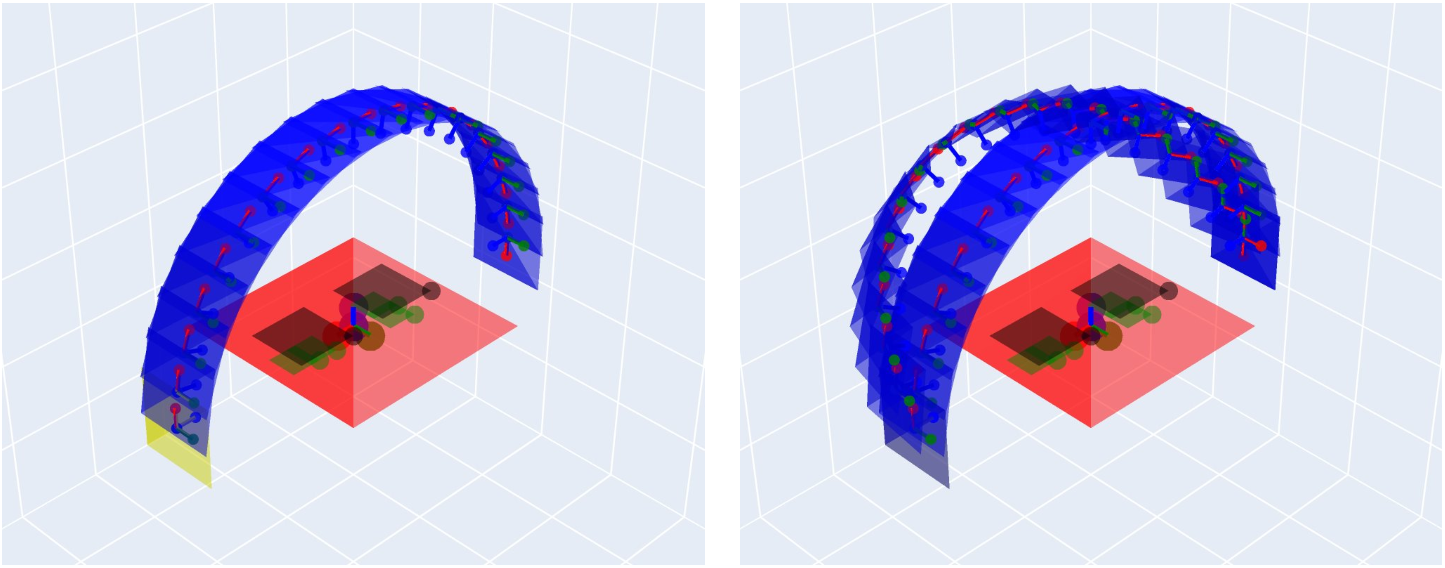
\includegraphics[width=0.8\textwidth]{chapters/methodology/SoftwareModel/images/Rigid Arc.png} % change {path}
    \caption{Rigid Arc Scanning Mode - Tilt Angles Left (0°) Right (0°,45°) }       % change {caption}
    \label{fig:Ridig Arc Scanning Mode}            % change label - used for reference in text
\end{figure}   

\paragraph{Horizontal Circles}

This method generates a set of circular paths in the XY plane, each at a different Z height ($\varphi$) angles:

\begin{itemize}
    \item At each Z-level (elevation), the plane performs a full 360° rotation around the Z-axis, visualised in left figure~\ref{fig:Horizontal and Vertical Scanning Modes}
    \item Simulating scanning the sensor area from different elevation angles, while keeping the plane parallel to the XY plane. 
\end{itemize}

\paragraph{Vertical Circles}

In this mode, the source moves along vertical arcs (meridians), while scanning across azimuthal ($\theta$) angles:

\begin{itemize}
    \item At each azimuthal angle, the plane performs a 180° rotation around the Z-axis visualised in right figure~\ref{fig:Horizontal and Vertical Scanning Modes}.
    \item This movement style traces vertical circles, like longitude lines on a globe.
\end{itemize}

\begin{figure}[htbp] %h-ere t-op b-ottom p-page (separte) -good to allow all htbp to give the compiler more options
    \centering
    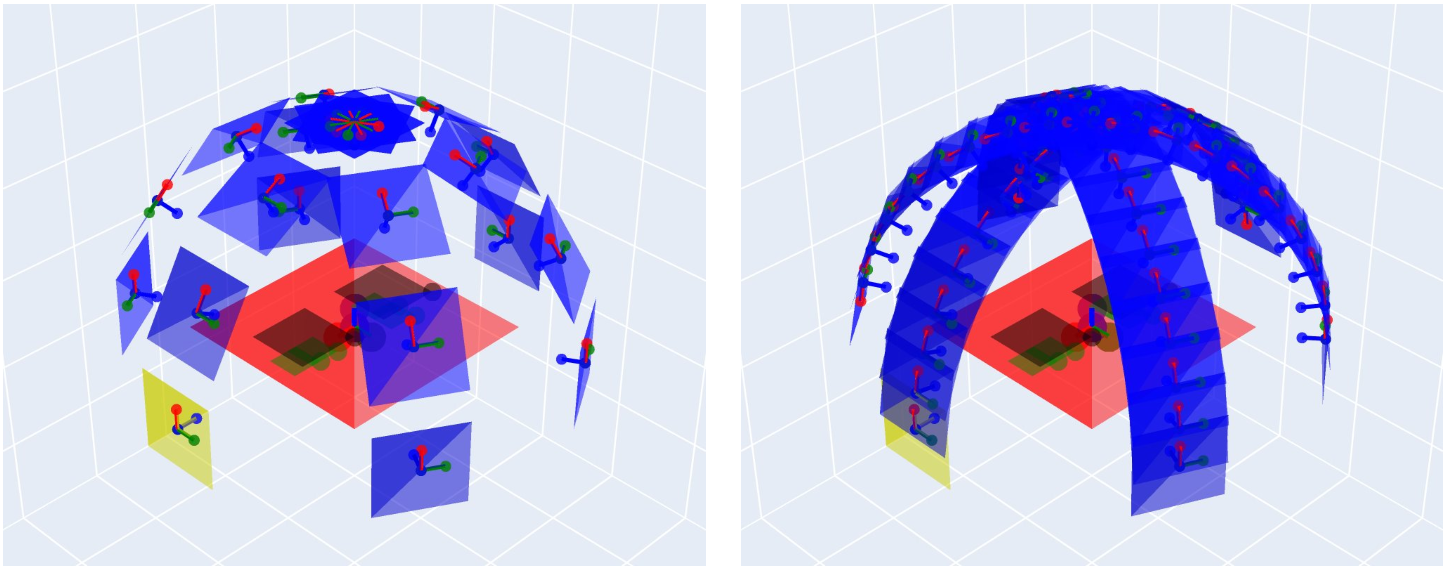
\includegraphics[width=0.8\textwidth]{chapters/methodology/SoftwareModel/images/Other movements.png} % change {path}
    \caption{Horizontal and Vertical Scanning Modes}       % change {caption}
    \label{fig:Horizontal and Vertical Scanning Modes}            % change label - used for reference in text
\end{figure}  

\subsubsection{Intersections}
The intersection calculations are implemented in the intersectionCalculations.py module, with four main functions:
\begin{lstlisting}[style=pythonstyle, caption=Ray-Plane Intersection Algorithm, label=lst:Ray-Plane Intersection Algorithm, language=Python ]
    def direction_vectors(vectorA, vectorB):
        """
        Calculates the dot product between two vectors.
        Used to check if ray direction and plane normal are parallel.
        Args:
            vectorA: First vector (Plane normal direction)
            vectorB: Second vector (Ray normal direction)
            
        Returns:
            Dot product of the two vectors
        """
        check_direction = np.multiply(vectorA, vectorB)
        check_direction = np.sum(check_direction)

    return check_direction

    def compute_t(nP, nA, nU):
        """
        Computes the parameter t in the line equation.
        Args:
            nP: Dot product of plane normal and plane position
            nA: Dot product of plane normal and line position
            nU: Dot product of plane normal and line direction
            
        Returns:
            Parameter t at which line intersects the plane
        """
    return (nP - nA) / nU

    def calculate_intersection(line, t):
        """
        Calculates the intersection point using the line equation.
        Args:
            line: Line object with position and direction
            t: Parameter value
            
        Returns:
            3D coordinates of the intersection point
        """
        x = line.direction[0] * t + line.position[0]
        y = line.direction[1] * t + line.position[1]
        z = line.direction[2] * t + line.position[2]

        coordinates = np.array([x,y,z])
    return coordinates

    def intersection_wrapper(sensorPlane, line1):
        """
        Coordinates the intersection calculation process.
        Args:
            sensorPlane: Plane object with position and normal
            line1: Line object with position and direction
            
        Returns:
            Intersection coordinates or None if no intersection exists
        """
        nU = direction_vectors(sensorPlane.direction, line1.direction)

        if nU != 0:
            nA = np.dot(sensorPlane.direction, line1.position)
            nP = np.dot(sensorPlane.direction, sensorPlane.position)

            x = compute_t(nP, nA, nU)
            IntersectionCoordinates = calculate_intersection(line1, x)

            return IntersectionCoordinates
        else:
            print(f" Intersection not possible for nU vector: {nU}")
            return None
\end{lstlisting}

After calculating the intersection point, the system checks if the point falls within the specified areas on the planes. This is handled by the \verb|record_result| method in the \verb|Areas| class:

\begin{lstlisting}[style=pythonstyle, caption=Area Intersection Testing, label=lst:Area_Intersection_Testing, language=Python ]
    def record_result(self, cords):
        """
        Determines if an intersection point falls within the area boundaries.
        Args:
            cords: 3D coordinates of the intersection point
            
        Returns:
            1 if point is within area (hit), 0 otherwise (miss)
        """
        # True if intersection x coordinate is within area boundary (x min and x max)
        if (self.position[0] - (self.width / 2) <= cords[0] <= self.position[0] + (self.width / 2)
                and  # True if intersection y coordinate is within area boundary (y min and y max)
                self.position[1] - (self.length / 2) <= cords[1] <= self.position[1] + (self.length / 2)):
            return 1
        else:
            return 0
    \end{lstlisting}

This process runs incrementally, checking whether the lines intersect with apertures, and if so, checking for intersection with sensors. If both conditions are met, then 'illumination' occurs. 

\paragraph{Assumptions}
The development of the software model and simulation framework involved several assumptions to enable tractable, consistent, and focused analysis. These assumptions are the basis for the implementation and set the boundary conditions for interpreting results.

\paragraph{Geometric}
\begin{itemize}
    \item Planes are rectangular and rigid: All $Plane$ and $Area$ objects are assumed to be flat rectangular surfaces.
    \item Local coordinate frames $(right, up, normal)$ are assumed to form an orthonormal basis derived via the $right-hand$ rule using a predefined $world_up$ vector.
    \item Plane local coordinates are recalculated from the center position and orientation at each step using fixed width and length.
\end{itemize}

\paragraph{Line Emission and Direction}
\begin{itemize}
    \item Lines are emitted orthogonally to the source plane’s surface (i.e., in the direction of the plane’s normal vector).

    \item All lines are assumed to be infinite in length, with intersection checked against finite planes.
    
    \item Initial emission points for all lines are randomly distributed within the local bounds of the source plane.
\end{itemize}

\paragraph{Rotation and Arc Movement}
\begin{itemize}
    \item In rigid arc mode, the plane always faces the global origin regardless of position.

    \item For vertical and horizontal circle modes:
    \item Planes move along spherical arcs with constant radius.
    \item Primary and secondary rotation matrices are sequentially applied using defined axes.
    \item Rotations are idealised and simplistic: Instantaneous and discrete.
\end{itemize}

\paragraph{Intersection Physics and Hit Detection}
\begin{itemize}
    \item Intersection detection assumes ideal mathematical planes: Thickness, reflectivity, or surface texture are not modelled.
    \item A line is marked as a hit only if the intersection point lies within both the aperture area and a defined sensor area.
    \item No consideration is given to beam divergence, attenuation, or scattering.
    \item No physical laws (e.g., Snell’s law) are implemented — the model uses only geometric approximation.
\end{itemize}

\subsubsection{Model Configuration}

A .JSON file is used to allow for easy setup of different experimental scenarios without modifying code:

\begin{itemize}
\item Detailed definition of planes, including position, orientation, and dimensions
\item Sensor and aperture areas with specific positions and sizes
\item Trajectory specifications for various movement types
\item Simulation parameters (number of rays, iterations)
\item Visualisation options - Static, or animated plot 
\item Debugging and performance settings
\end{itemize}

The \texttt{Config} class (Listing~\ref{lst:Model_Config_code}) loads and parses the configuration file, making parameters accessible throughout the application:
\begin{lstlisting}[style=pythonstyle, caption=Model configuration - Config Class, label=lst:Model_Config_code, language=Python ]
    
    class Config:
        def init(self, file_path=None, data=None):
        if data is not None:
        self.load_from_dict(data)
        elif file_path:
        with open(file_path, "r") as f:
        data = json.load(f)
        self.load_from_dict(data)
        else:
        raise ValueError("Must provide either file_path or data")
    
    def load_from_dict(self, data):
        self.planes = data["planes"]
        self.sensor_areas = data["sensor_areas"]
        self.aperture_areas = data["aperture_areas"]
        self.arc_movement = data["arc_movement"]
        self.simulation = data["simulation"]
        self.intersection = data["intersection"]
        self.visualization = data["visualization"]
        self.debugging = data["debugging"]
        self.performance = data["performance"]
        self.output = data["output"]
    \end{lstlisting}

Additionally available to the user is an interface, allowing for easy manipulation of the parameters, and visual representation of the sensor positions. Figure~\ref{fig:Model Configuration Interface} 

\begin{figure}[htbp] %h-ere t-op b-ottom p-page (separte) -good to allow all htbp to give the compiler more options
    \centering
    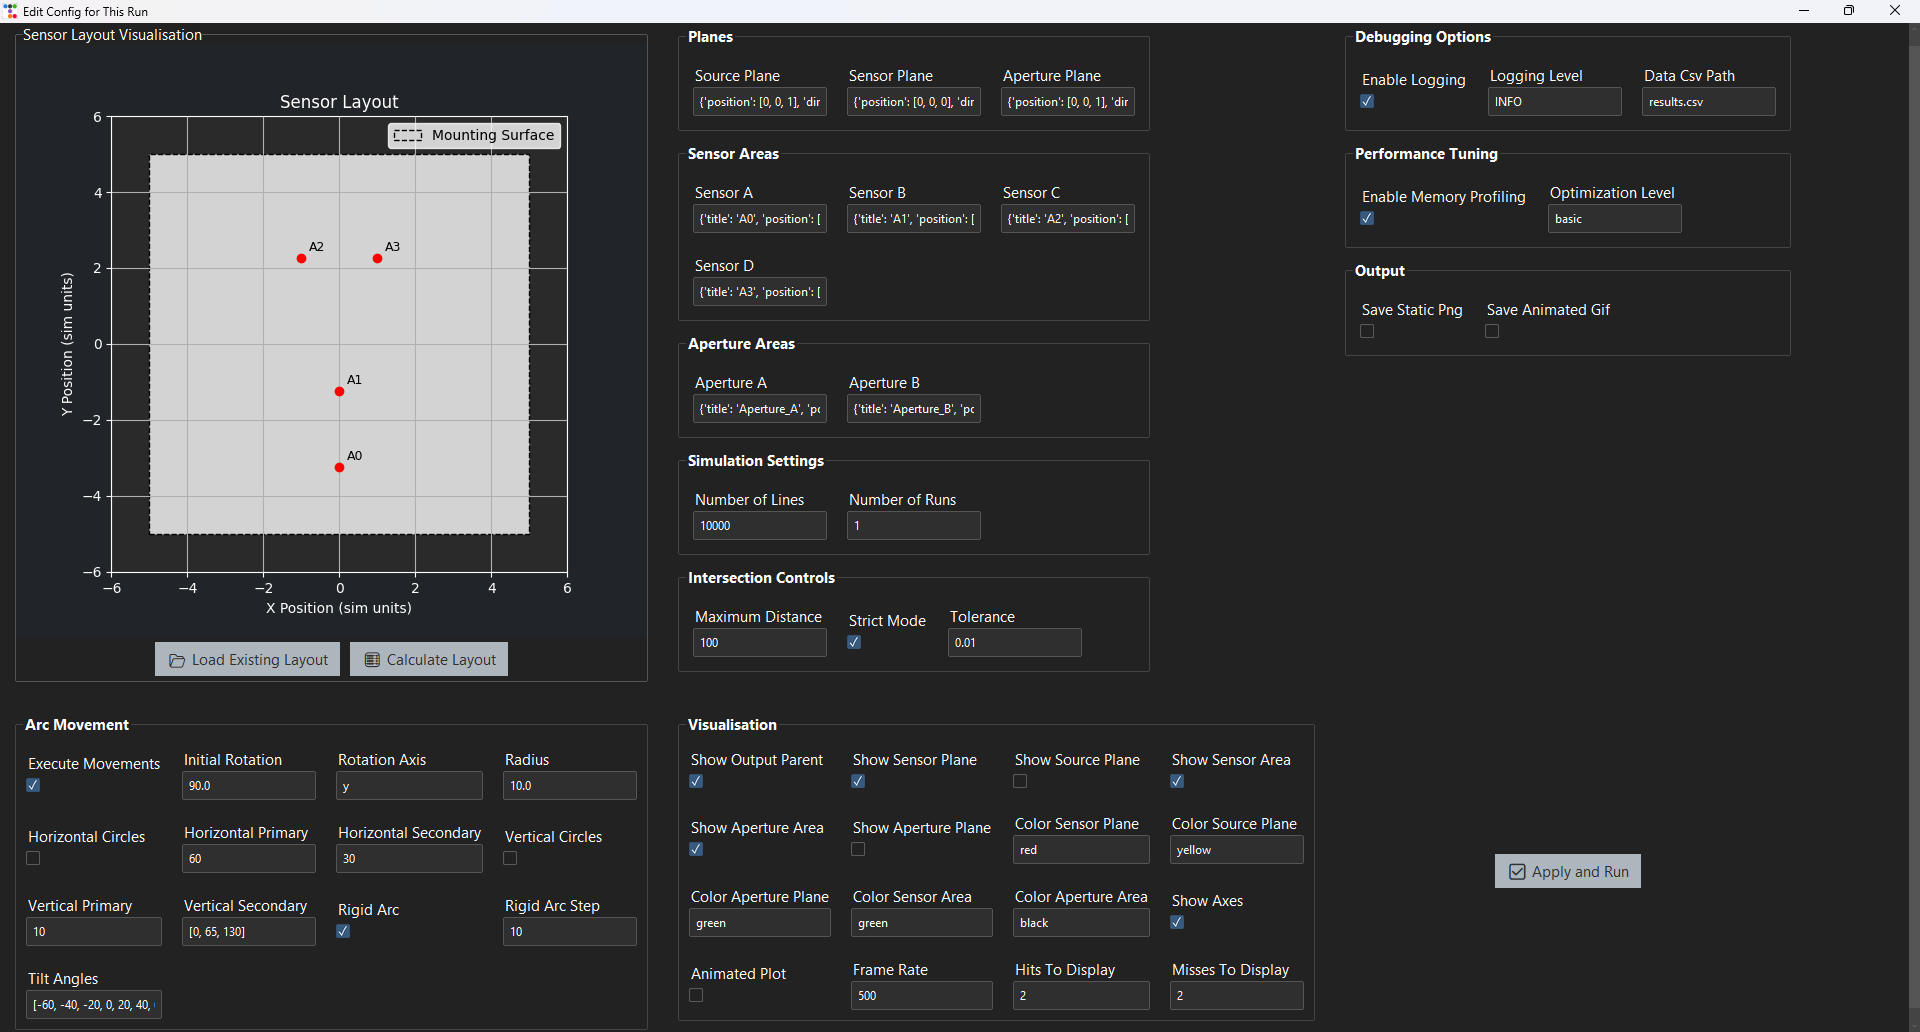
\includegraphics[width=0.8\textwidth]{chapters/methodology/SoftwareModel/images/Interface.png} % change {path}
    \caption{Model Configuration Interface}       % change {caption}
    \label{fig:Model Configuration Interface}            % change label - used for reference in text
\end{figure}                             % for example: see in Figure~\ref{example label}


\subsubsection{Model Output}
The simulation calculates how many light rays (lines) emitted from a movable source plane are successfully transmitted through the apertures and reach specific sensor areas. This output is stored in CSV files.

\paragraph{$results.csv$}

This file records summary statistics for each simulated position during the arc movement, containing:

\begin{table}[h]
    \centering
    \caption{Simulation Output: Summary of Each Arc Position}
    \label{tab:simulation_results_csv}
    \begin{tabular}{>{\raggedright\arraybackslash}p{2.5cm}>{\centering\arraybackslash}p{3cm}>{\raggedright\arraybackslash}p{6cm}}
    \toprule
    \textbf{Field} & \textbf{Example} & \textbf{Description} \\
    \midrule
    sim & 0 & Simulation run index \\
    idx & 4 & Arc position index (step in movement sequence) \\
    hits & 6321 & Number of rays that reached any sensor area \\
    misses & 3679 & Number of rays that missed all sensors \\
    ray count & 10000 & Total rays emitted during this simulation run \\
    sim title & Basic & Custom label identifying the simulation configuration \\
    runtime & 1.2847 & Execution time (seconds) for this movement type \\
    \bottomrule
    \end{tabular}
\end{table}

Providing overall results for any given simulation run.

\paragraph{$sensor\_results.csv$}

This file records individual sensor readings for each simulated position, containing:

\begin{table}[h]
    \centering
    \caption{Sensor Output: Ray Hits Per Sensor at Each Arc Position}
    \label{tab:sensor_results_csv}
    \begin{tabular}{>{\raggedright\arraybackslash}p{2.5cm}>{\centering\arraybackslash}p{3cm}>{\raggedright\arraybackslash}p{6cm}}
    \toprule
    \textbf{Field} & \textbf{Example} & \textbf{Description} \\
    \midrule
    sim & 0 & Simulation run index \\
    idx & 4 & Arc position index (step in movement sequence) \\
    A0 & 2450 & Number of rays hitting Sensor A0 \\
    A1 & 1783 & Number of rays hitting Sensor A1 \\
    A2 & 1044 & Number of rays hitting Sensor A2 \\
    A3 & 1044 & Number of rays hitting Sensor A3 \\
    \bottomrule
    \end{tabular}
\end{table}
